\resizebox{0.4
\textwidth}{!}{%
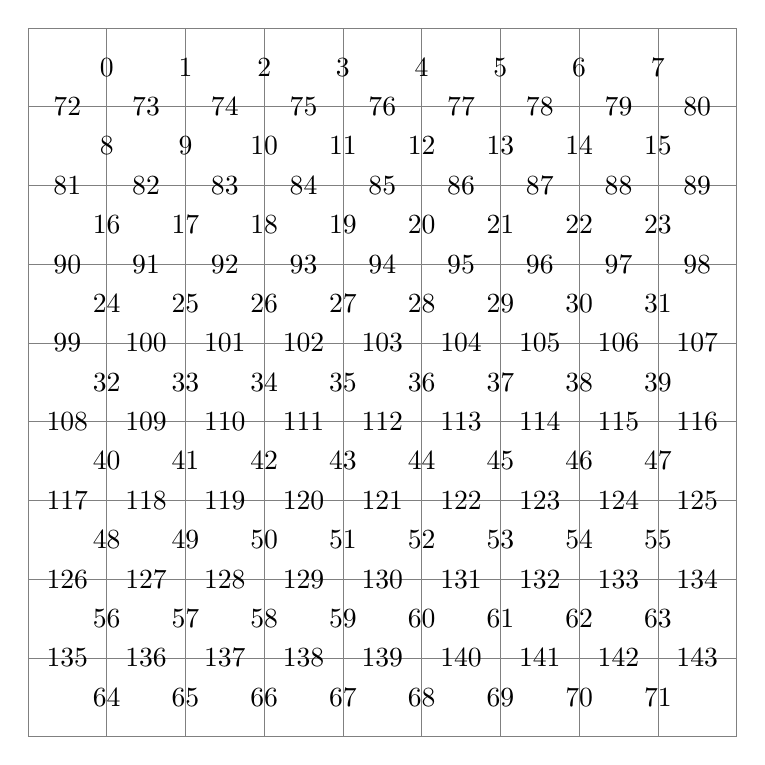
\begin{tikzpicture}[]
\draw[step=1cm,gray,very thin] (0,0) grid (9,9);

\foreach \x in {1,2,3,4,5,6,7,8}{
    \foreach \y [evaluate=\y as \index using int(\x-1+(\y-1)*8)] in {1,2,3,4,5,6,7,8,9}{
        \node at (\x, 9.5 - \y) {\index};
    }
}

\foreach \x in {1,2,3,4,5,6,7,8,9}{
    \foreach \y [evaluate=\y as \index using int(71+\x+(\y-1)*9)] in {1,2,3,4,5,6,7,8}{
        \node at (\x - 0.5, 9-\y) {\index};
    }
}

\end{tikzpicture}
}